\documentclass[12pt]{article}

%\usepackage[dvips]{graphics,color}
\usepackage{fullpage}
%\usepackage{amsfonts}
\usepackage{amssymb}
\usepackage{amsmath}
%\usepackage{latexsym}
\usepackage{enumerate}
\usepackage{fancybox}
\usepackage{float}
\usepackage{tikz}
\usepackage{gensymb}
\usepackage{units}
\usepackage{ifthen}
\usetikzlibrary{calc}
\usetikzlibrary{automata,positioning}
\pagenumbering{gobble}

\usepackage{graphicx}
\graphicspath{{./}}
\usepackage{wrapfig}
\DeclareGraphicsExtensions{.png,.jpg}

\setlength{\parskip}{1pc}
\setlength{\topmargin}{-1pc}
\setlength{\textheight}{9in}

\begin{document}
\begin{center}
{\Large CS244 PA3 Intermediate Progress Report}
\begin{center}
Gus Liu, Eli Berg - Spring 2016 \\
sunetids: gusliu, ejberg
\end{center} 
\end{center}

\section*{Goals}	
	This paper, \textit{Queues don't matter when you can JUMP them!} was presented by Matthew P. Grosvenor et al. at NSDI 2015 as an algorithm for mitigating the effects of network congestion due to cross-application interference in datacenters. It aims to enforce the often stated trade off between high throughput needs and low latency guarantees by coupling the two in a software rate limiter. The underlying idea is that a latency sensitive application, such as PTPd or memcached, should be willing to accept stricter rate limits in exchange for a higher packet priority, while high throughput applications such as Hadoop would make the opposite trade-off. Their discussion of "maximum fan-in" concludes that we can bound the expected possible latency of a network in any given epoch by the ingress to a single end host if every other host on the network could potentially attempt to communicate with that one simultaneously. This is a nice conclusion because it means that an arbitrarily complex datacenter network can be modeled as a single shared switch in which several attached hosts attempt to communicate with one host via a single link. 

\section*{Motivation}
	Many datacenter applications are sensitive to tail latencies, demonstrating the need for QJump to reduce network interference. When users experience high latency, companies lose out on user engagement and potential revenue significantly. Moreover, QJump is designed to be immediately deployable and simple, requiring no change to hardware or application code. The authors found in preliminary experiments that latency-sensitive applications can degrade in performance from 16x to 85x worse when sharing the network at various places with a throughput-intensive bulk transfer application. The authors concluded that there is clearly much room for improvement when users would like to improve the performance of those latency-sensitive applications with minimal sacrifice to high throughput applications.
	
\section*{Results}
	The authors found that QJump exhibits better interference control than existing schemes such as ECN or DCTCP. The variance in Hadoop, PTPd and memcached performance is close to (Hadoop, PTPd) or slightly better than (memcached) in the uncontended ideal case. Moreover, QJump provides excellent overall average and 99th percentile flow completion times. It performed best on short flows, although it achieves similar or better results than pFabric on average and 99th percentile FCTs. However, on large flows, the results are mixed. 
	
\section*{Subset Goal and Motivation}
	We propose to implement the QJump rate limiter as a traffic control module in the Linux kernel as was done in the paper. We then aim to reproduce the experiment shown in figure 5, in which PTPd and memcached are run over an otherwise empty network both with and without a currently running Hadoop job. We may scale down their test topology to something like 6 hosts and 3 switches, or even a few hosts connected to a single switch and sending traffic over the same output link to a single end host. We hope to see the addition of QJump to the hosts eliminate the noticeable effects of a running Hadoop job as shown in the paper. The priorities (or $f$ values) can be hard-coded into a port mapping so we don't have to also implement the application utility that they talk about in the paper. If the kernel module proves particularly troublesome or intractable in the time we have, we could potentially fall back to an application-level rate limiter with more customizable traffic sources to play nice with application level traffic control. Mininet seems like an appropriate choice for virtualizing their experimental topology. This topology is considerably more reproducible in a virtualized environment than a complete datacenter topology.
	
	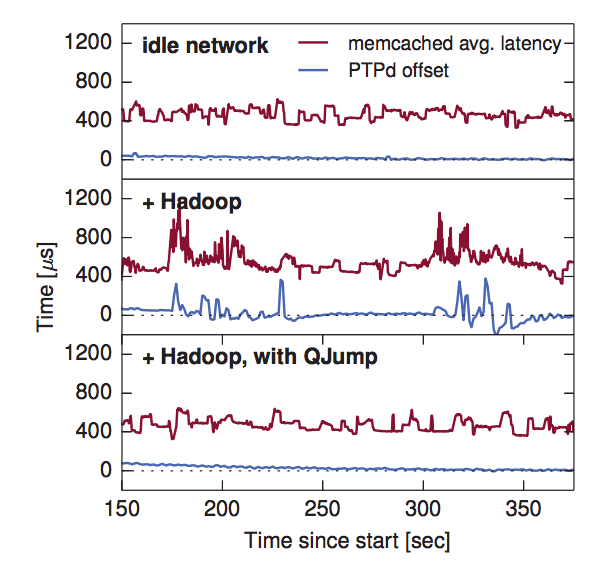
\includegraphics[width=200pt]{qjump.png} 
	
\section*{Current Progress}
	We have set up the network topology as described by the paper in Mininet. 
		
\end{document}




